\section {Gen and Kill Sets}
\setlength{\parindent}{0pt}
(Prepared by Sameer V. Pande)

\subsection{Transfer and Meet Functions}
In previous module we discussed about how a DFA can be expressed with help of transfer and meet functions.
Transfer function computes the value of out[s] as a function f(in[s]). And for forward dfa, when there are multiple incoming edges at a node,
the meet operator computes the in[s] as a function of outsets of the predecessors.

\subsection{Using GEN and KILL sets to represent transfer functions}
In most cases, it is possible to represent transfer function with help of gen-sets and kill-sets which depend only on the statement (hence, can be computed statically).
Transfer function 'f' can be written as: \textbf{f(V) = (V - Kill(s)) $\bigcup$ Gen(s)}. The first part of expression
\textbf{ V - Kill(S)} is called "propagate" part and \textbf{Gen(S)} is called 'generate' part.

\subsection{Examples of Gen and Kill Sets}
We'll see two examples of gen/kill sets 
\subsubsection{Constant Propataion}
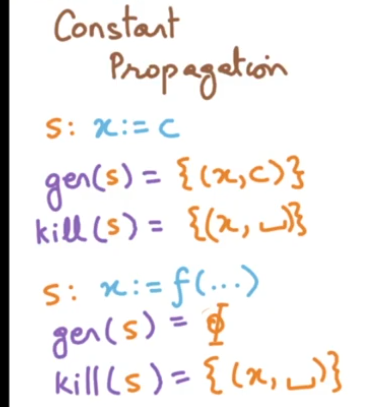
\includegraphics[scale=0.5]{images/89_1.png}
\newline 
The gen-set for constant-assignment is just \{(x,c)\}. The kill-set ensures that any previous value of the variable x is removed from the set, before new value is added via gen.
When x is assigned a value via a complex function/expression, then gen-set is empty-set but kill-set removes the old value of x, if any.
\subsubsection{Available Expressions Analysis}
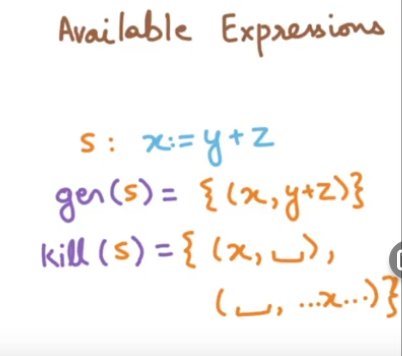
\includegraphics[scale=0.5]{images/89_2.png}
\newline 
Consider case when variable x is assigned an expression. The gen-set is similar to that of constant propgation (but now it has expressions as well, instead of just constants). The kill-set takes care of two things 
\begin{enumerate}
    \item Remove the expressions corresponding to variable x 
    \item Remove the variables which have expressions corresponding to older-value of x.
\end{enumerate}

\subsection{Gen/Kill Summaries for Basic Blocks}
One of the advantages of using basic-blocks is that it generates summaries over the entire block. We can take a sequential composition of transfer function of all statements in the basic-block to give us a block-level transfer function.
A block level transfer function can be represented using block level genset and killset.
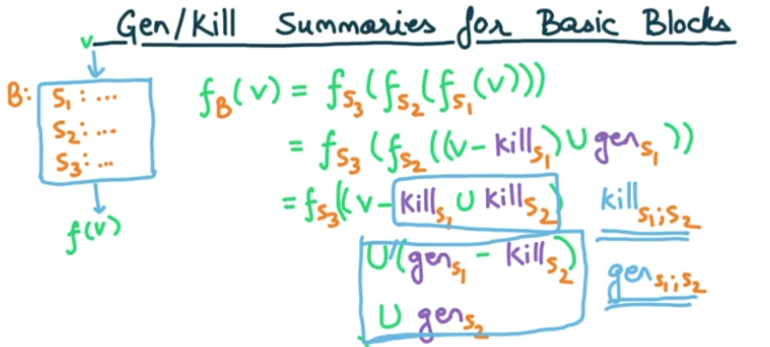
\includegraphics[scale=0.5]{images/89_3.png}

For a basic block B, Gen$_B$ and Kill$_B$ can be interpreted as follows:
\begin{itemize}
    \item Gen$_B$: Locally exposed constant definitions,i.e., the definitions available at the end of basic-block B.
    \item Kill$_B$: Set of constant definitions killed by B.
\end{itemize}